\documentclass[12pt]{article}
\usepackage[a4paper, total={6in, 9in}]{geometry}
\usepackage{graphicx}
\graphicspath{ {./images/output/} }
\usepackage{caption}
\usepackage[english]{babel}
\usepackage{titling}
\usepackage{float}
% \usepackage{amsmath}
% \usepackage{minted}
% \usepackage{multicol}
% \usepackage{array}
% \usepackage{setspace}
% \usepackage{placeins}

% \usepackage{lipsum}

\title{Study of Buck Converter Using Simulink}
\author{}
\date{}

\pagenumbering{gobble}
\begin{document}
\vspace*{\fill}
\begin{center}

    \emph{Heaven's Light is Our Guide} \\
    \textbf{Rajshahi University of Engineering and Technology} \\

    \begin{figure}[H]
        \centering
        
\includegraphics[scale=.34]{images/RUET_logo.png}
        \label{fig:ruet_logo}
    \end{figure}
    \vspace{5mm}

    \textbf{Course Code}\\
    ECE 3206\\
    \vspace{3mm}
    \textbf{Course Title}\\
    Industrial Electronics Sessional

    \vspace{5mm}
    \textbf{Experiment Date:} {January 13, 2025},\\
    \textbf{Submission Date:} {February 10, 2025}\\

    \vspace{5mm}
    \textbf{Lab Report 3: \\
        Study of Thyristor Characteristics R, RL Load}

    \vspace{15mm}

    \begin{tabular}{c|c}
        \textbf{Submitted to} & \textbf{Submitted by} \\
        Md. Faysal Ahamed     & Md. Tajim An Noor     \\
        Lecturer              & Roll: 2010025         \\
        Dept of ECE, Ruet     &                       \\
    \end{tabular}

\end{center}
\vspace*{\fill}


\pagebreak

\tableofcontents

\pagebreak
\pagenumbering{arabic}
\maketitle

\section*{Theory}
\addcontentsline{toc}{section}{Theory}
The Buck Converter is a DC-DC power electronic circuit that steps down the input voltage to a lower output voltage while maintaining high efficiency. It is widely used in applications such as power supplies, battery chargers, and voltage regulation in electronic devices \cite{rashid2013power}.

\subsection*{Working Principle}
The Buck Converter operates by switching a transistor on and off at high frequency. When the transistor is on, the input voltage is applied to the inductor, causing the current to increase. When the transistor is off, the inductor maintains the current flow through a diode and the load. The output voltage is determined by the duty cycle of the switching signal \cite{sen1987principles}.

\subsection*{Key Components}
\begin{itemize}
    \item Switching Transistor: Controls the on/off state of the circuit.
    \item Diode: Provides a path for the inductor current when the transistor is off.
    \item Inductor: Stores energy and smooths the current.
    \item Capacitor: Reduces voltage ripple at the output.
    \item Pulse Width Modulation (PWM) Controller: Regulates the duty cycle to achieve the desired output voltage.
\end{itemize}

\subsection*{Operation Modes}
\begin{itemize}
    \item Continuous Conduction Mode (CCM): The inductor current never falls to zero during operation.
    \item Discontinuous Conduction Mode (DCM): The inductor current falls to zero during part of the switching cycle.
\end{itemize}

\subsection*{Applications}
\begin{itemize}
    \item Voltage regulation in electronic devices
    \item Battery-powered systems
    \item Renewable energy systems
    \item Automotive electronics
\end{itemize}

MATLAB/Simulink simulations provide a powerful tool for analyzing the performance of the Buck Converter under various operating conditions, enabling optimization for specific applications \cite{mathworks2023simulink}.


\section*{Required Equipments/Software}
\addcontentsline{toc}{section}{Required Equipments/Software}
\begin{itemize}
    \item MATLAB/Simulink
    \item AC Voltage Source
    \item Thyristors (2 in anti-parallel configuration)
    \item Resistive Load (R)
    \item Inductive Load (RL)
    \item Pulse Generator for firing angle control
    \item Measurement Blocks (Voltage and Current)
    \item Scope for waveform visualization
\end{itemize}

\section*{Circuit Diagrams}
\addcontentsline{toc}{section}{Circuit Diagrams}
\begin{figure}[H]
    \centering
    % 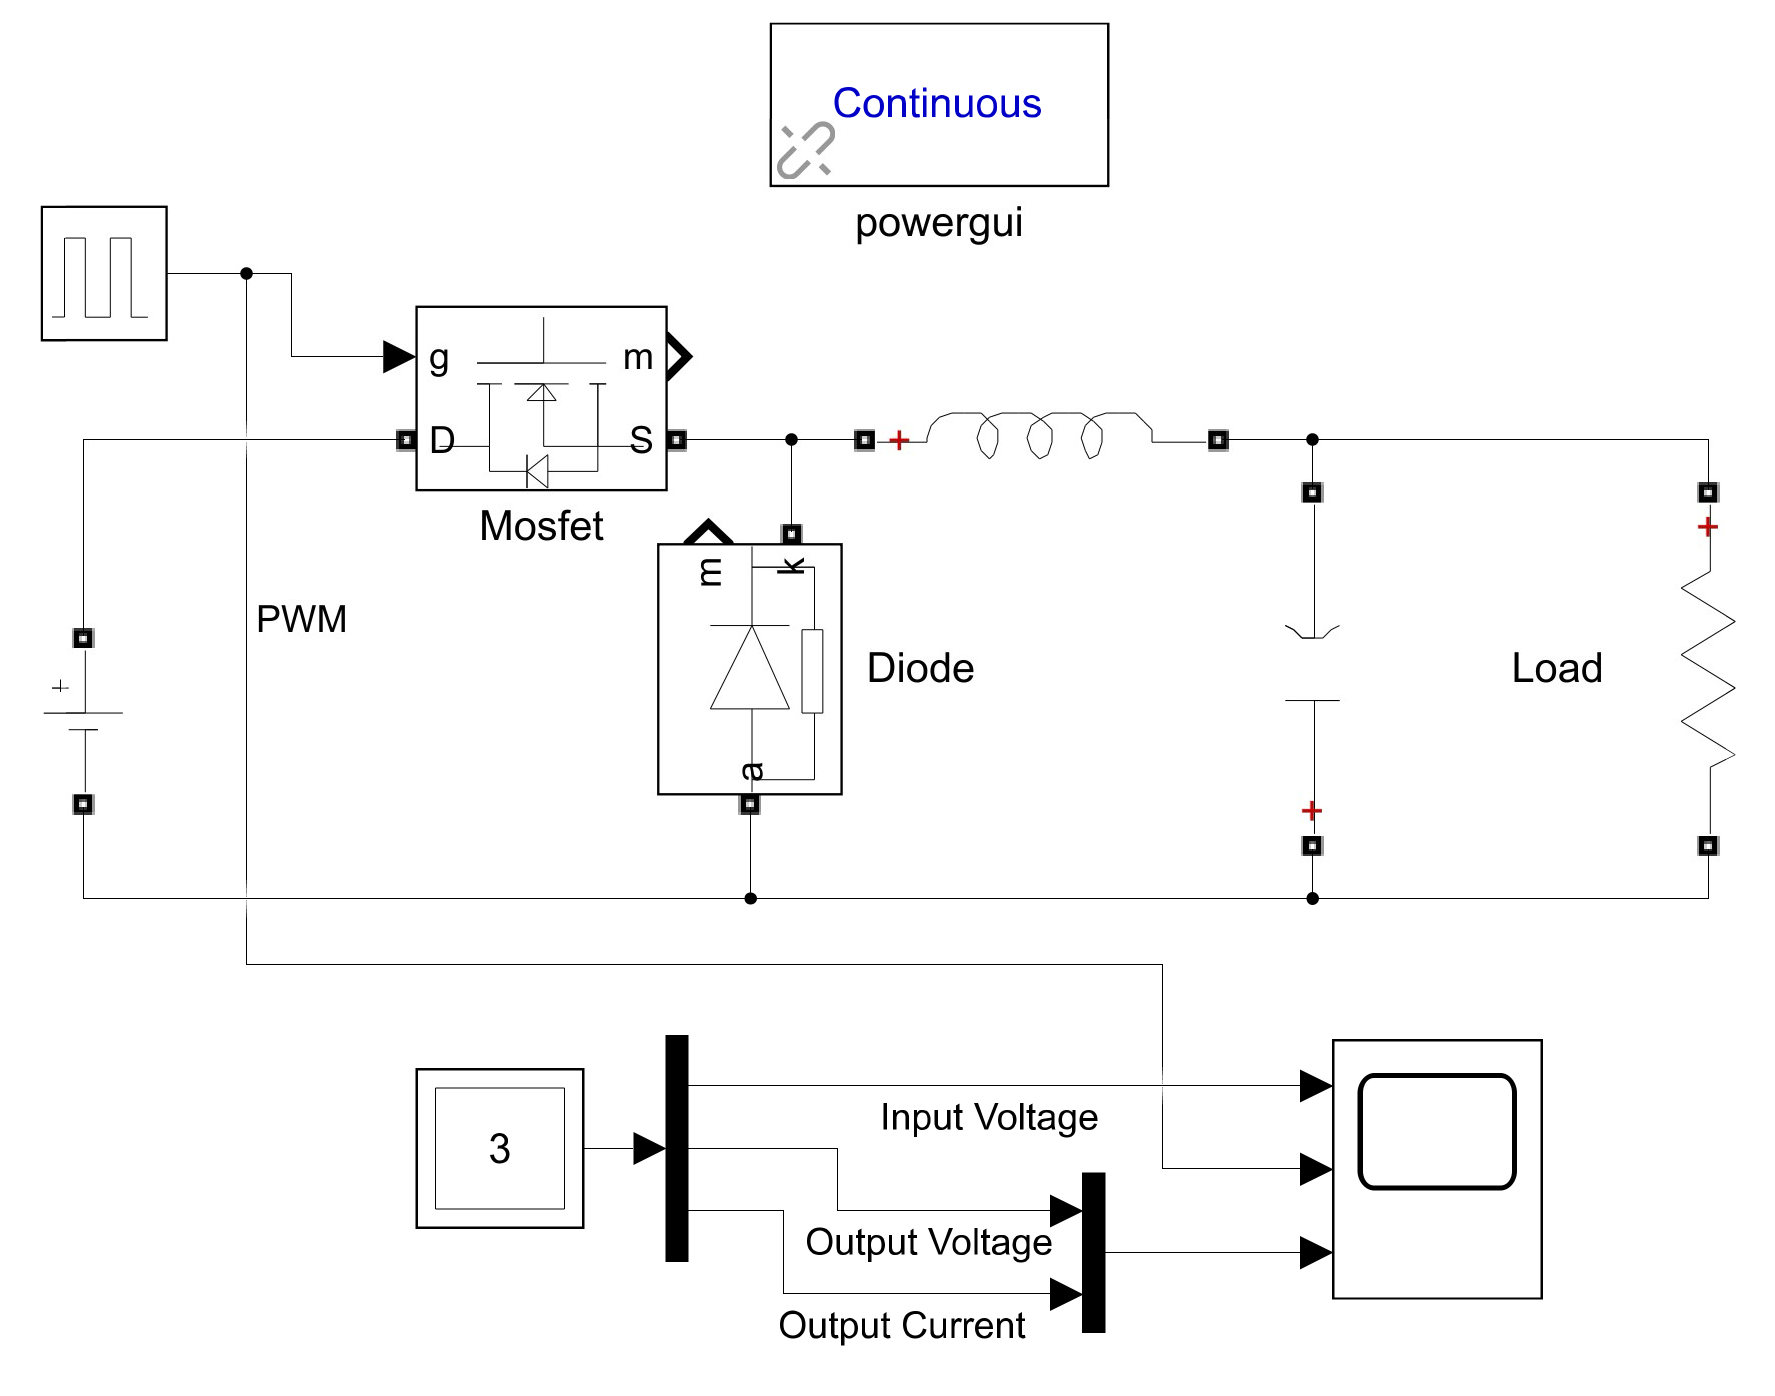
\includegraphics[width=\textwidth]{ckt.png}
    \caption{DC-DC Buck Converter Circuit Diagram}
\end{figure}

\section*{Observations}
\addcontentsline{toc}{section}{Observations}
\begin{itemize}
    \item For the Buck Converter, the output voltage is directly proportional to the duty cycle of the PWM signal.
    \item Increasing the duty cycle results in a higher output voltage, while decreasing it reduces the output voltage.
    \item In Continuous Conduction Mode (CCM), the inductor current never falls to zero, ensuring smooth operation and reduced ripple.
    \item In Discontinuous Conduction Mode (DCM), the inductor current falls to zero during part of the switching cycle, leading to increased ripple.
    \item MATLAB/Simulink simulations demonstrate the relationship between duty cycle, output voltage, and inductor current under various load conditions.
    \item The circuit effectively steps down the input voltage to the desired level with high efficiency.
    \item The results highlight the importance of proper component selection and PWM control for optimal performance in Buck Converter applications.
\end{itemize}


\subsubsection*{Outputs}
\begin{figure}[H]
    \centering
    % 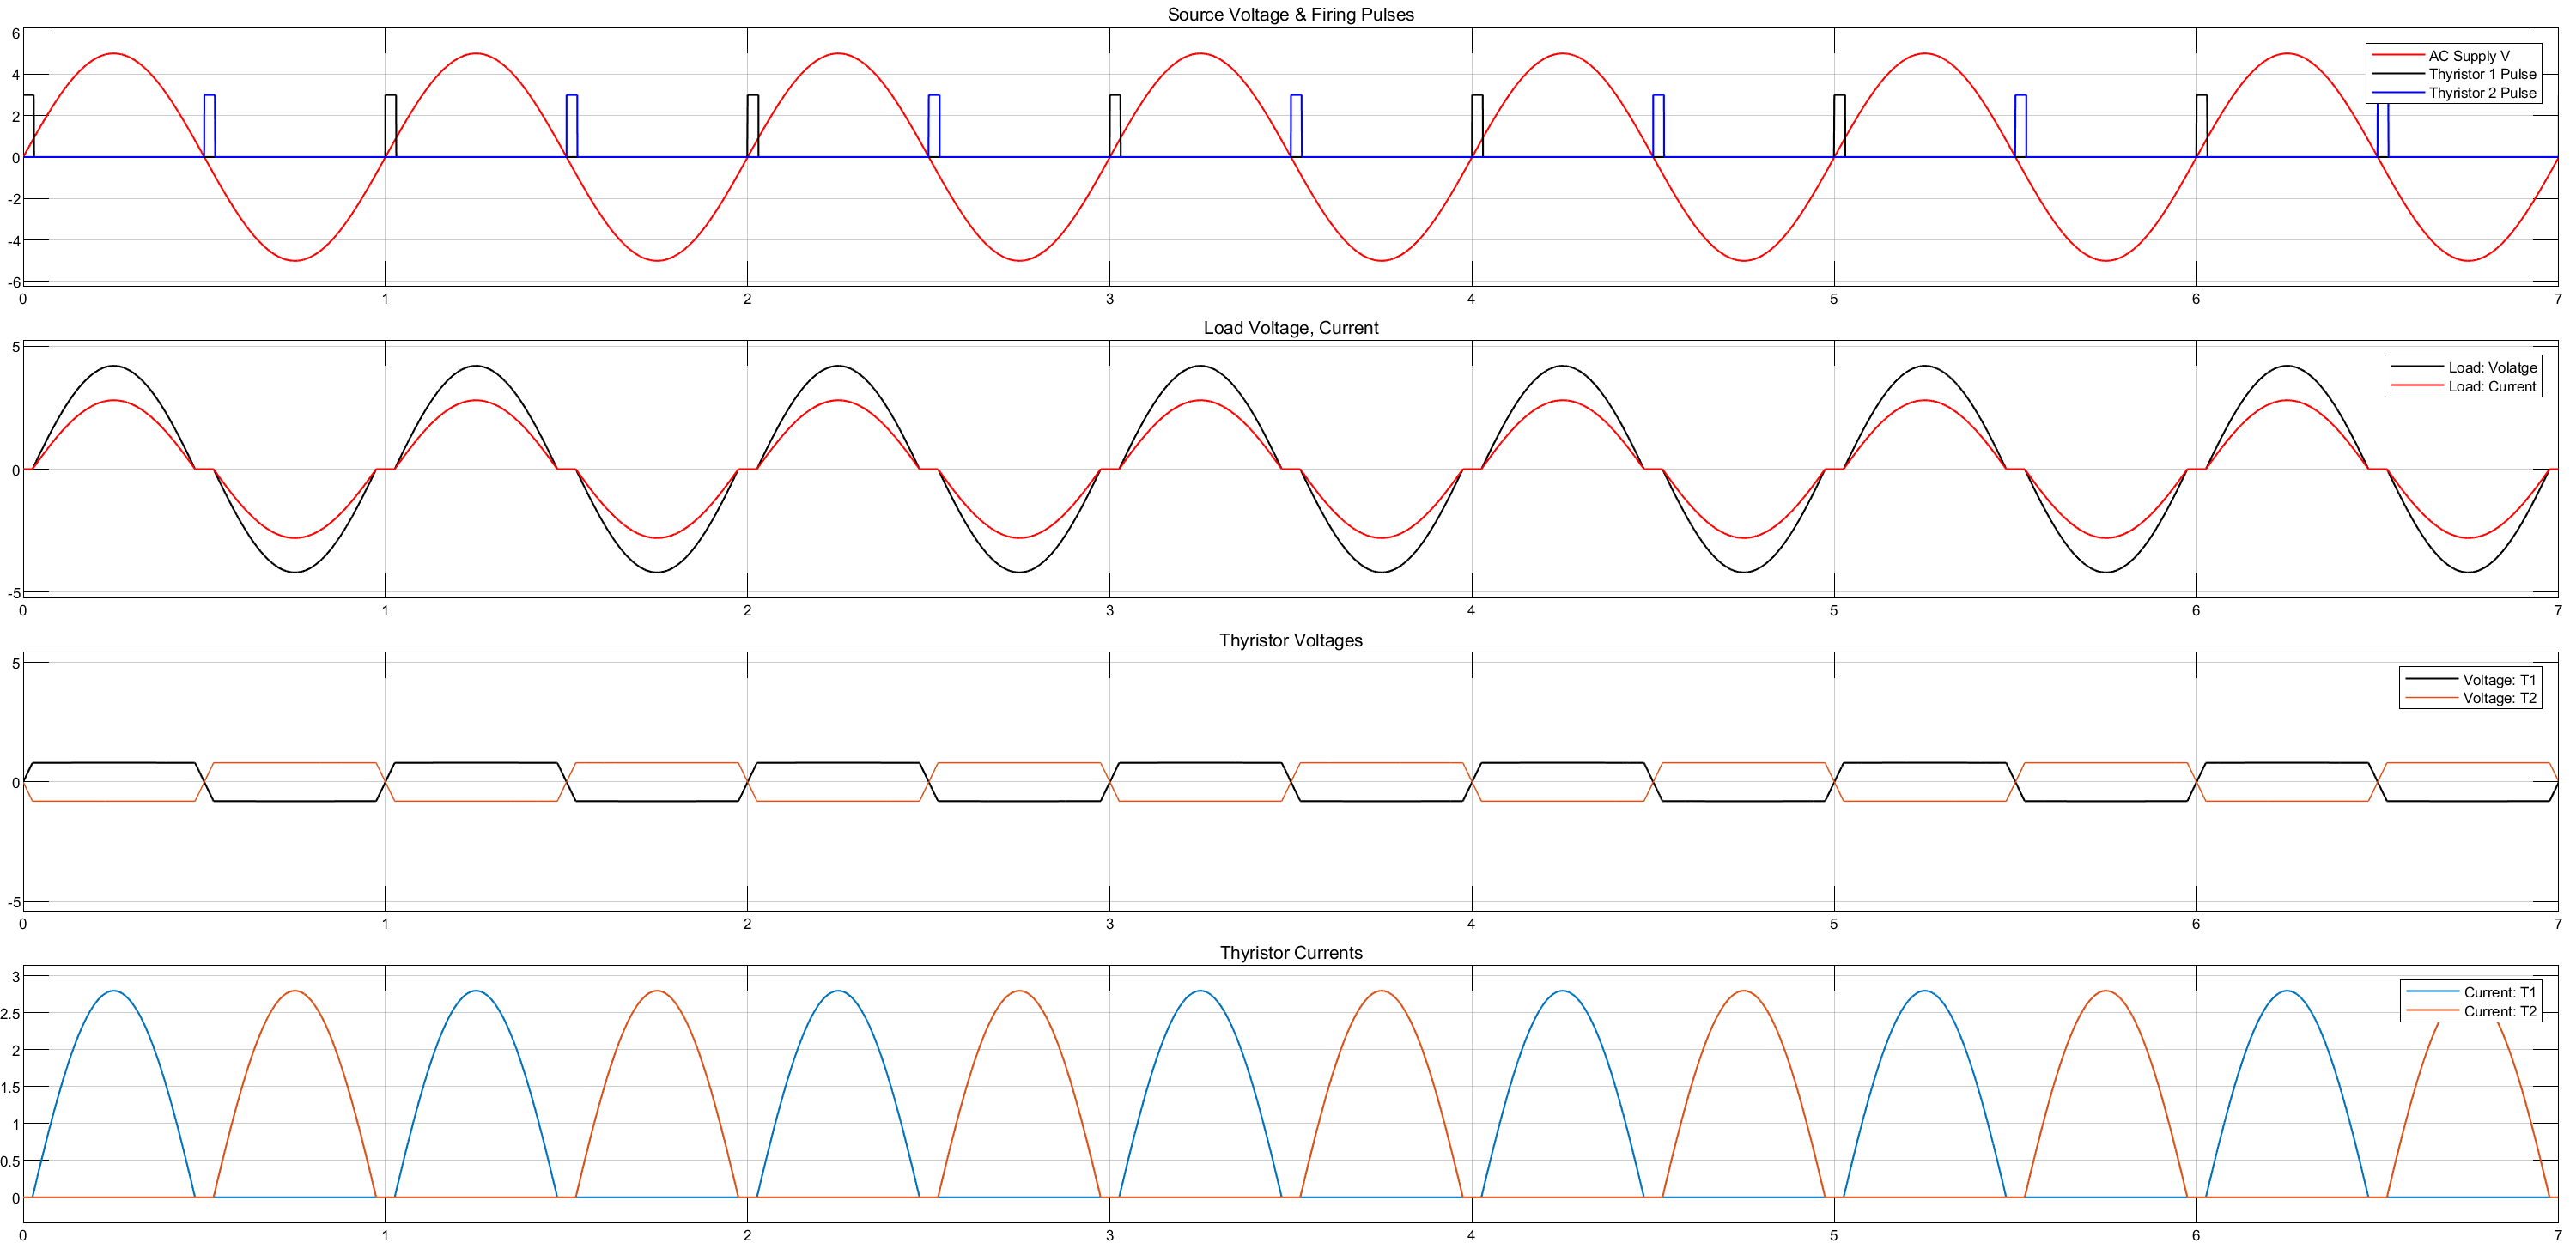
\includegraphics[width=\textwidth]{1Rnd.png}
    \caption{Simulation Output for R Load, Controlled Rectifier, No Delay}
    \label{fig:rControlledNoDelay}
\end{figure}

\begin{figure}[H]
    \centering
    % 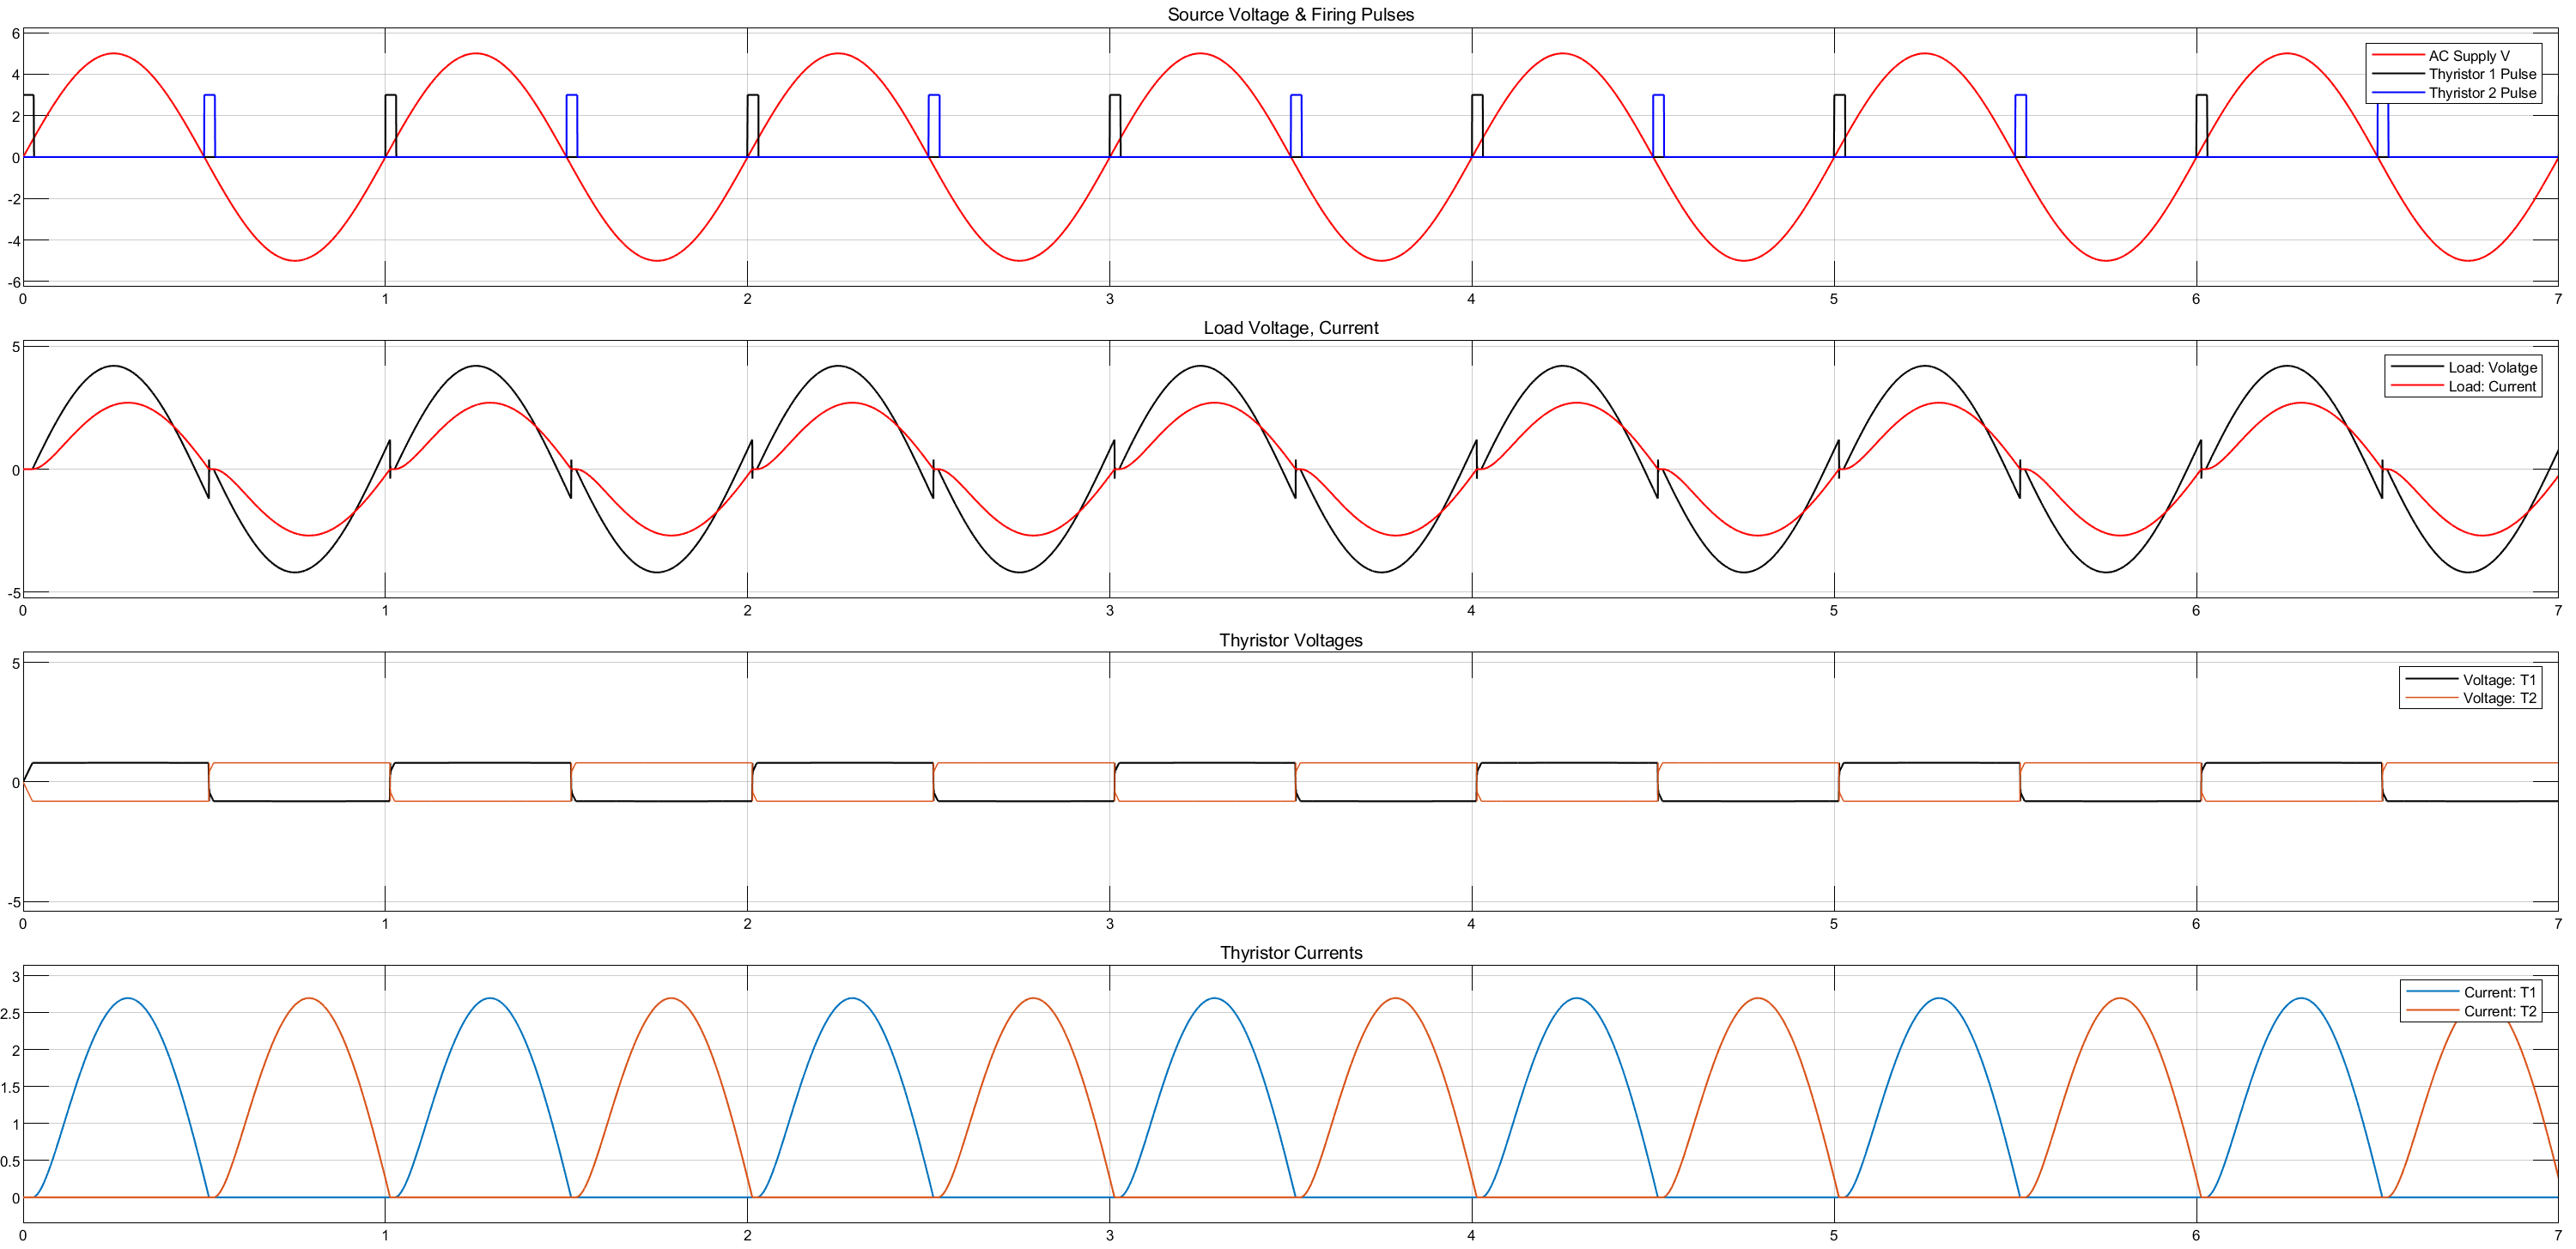
\includegraphics[width=\textwidth]{2RLnd.png}
    \caption{Simulation Output for RL Load, Controlled Rectifier, No Delay}
    \label{fig:rControlledWithDelay}
\end{figure}

\begin{figure}[H]
    \centering
    % 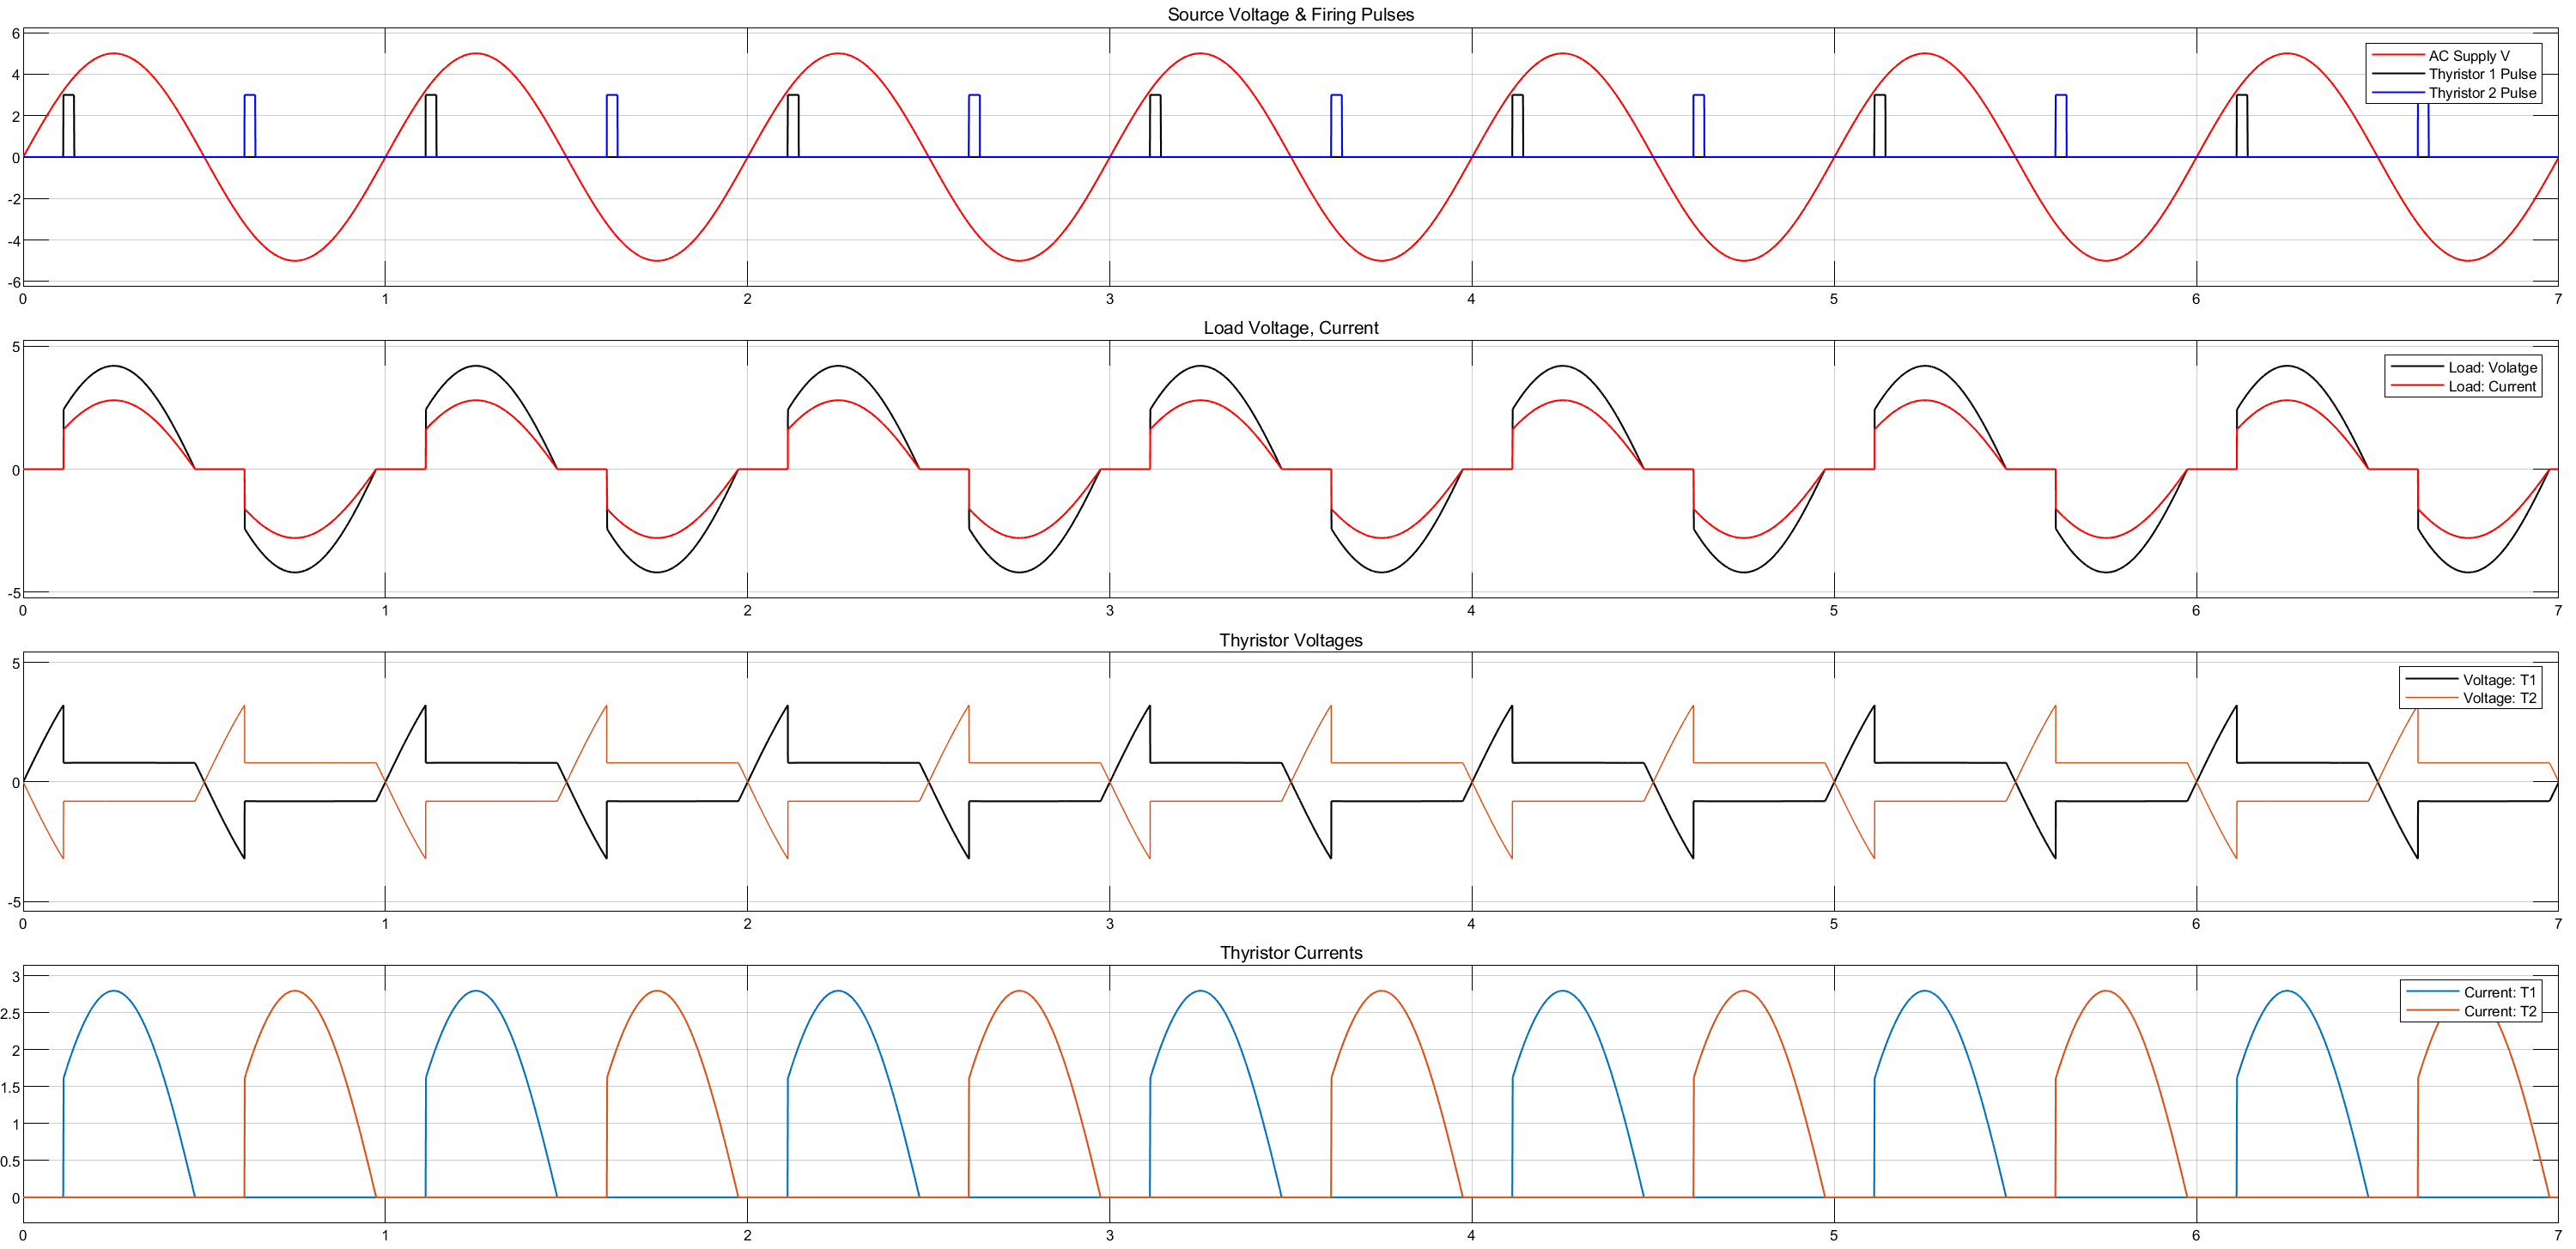
\includegraphics[width=\textwidth]{3Rd.png}
    \caption{Simulation Output for R Load, AC-AC Bidirectional Voltage Controller}
    \label{fig:rLoad}
\end{figure}

\begin{figure}[H]
    \centering
    % 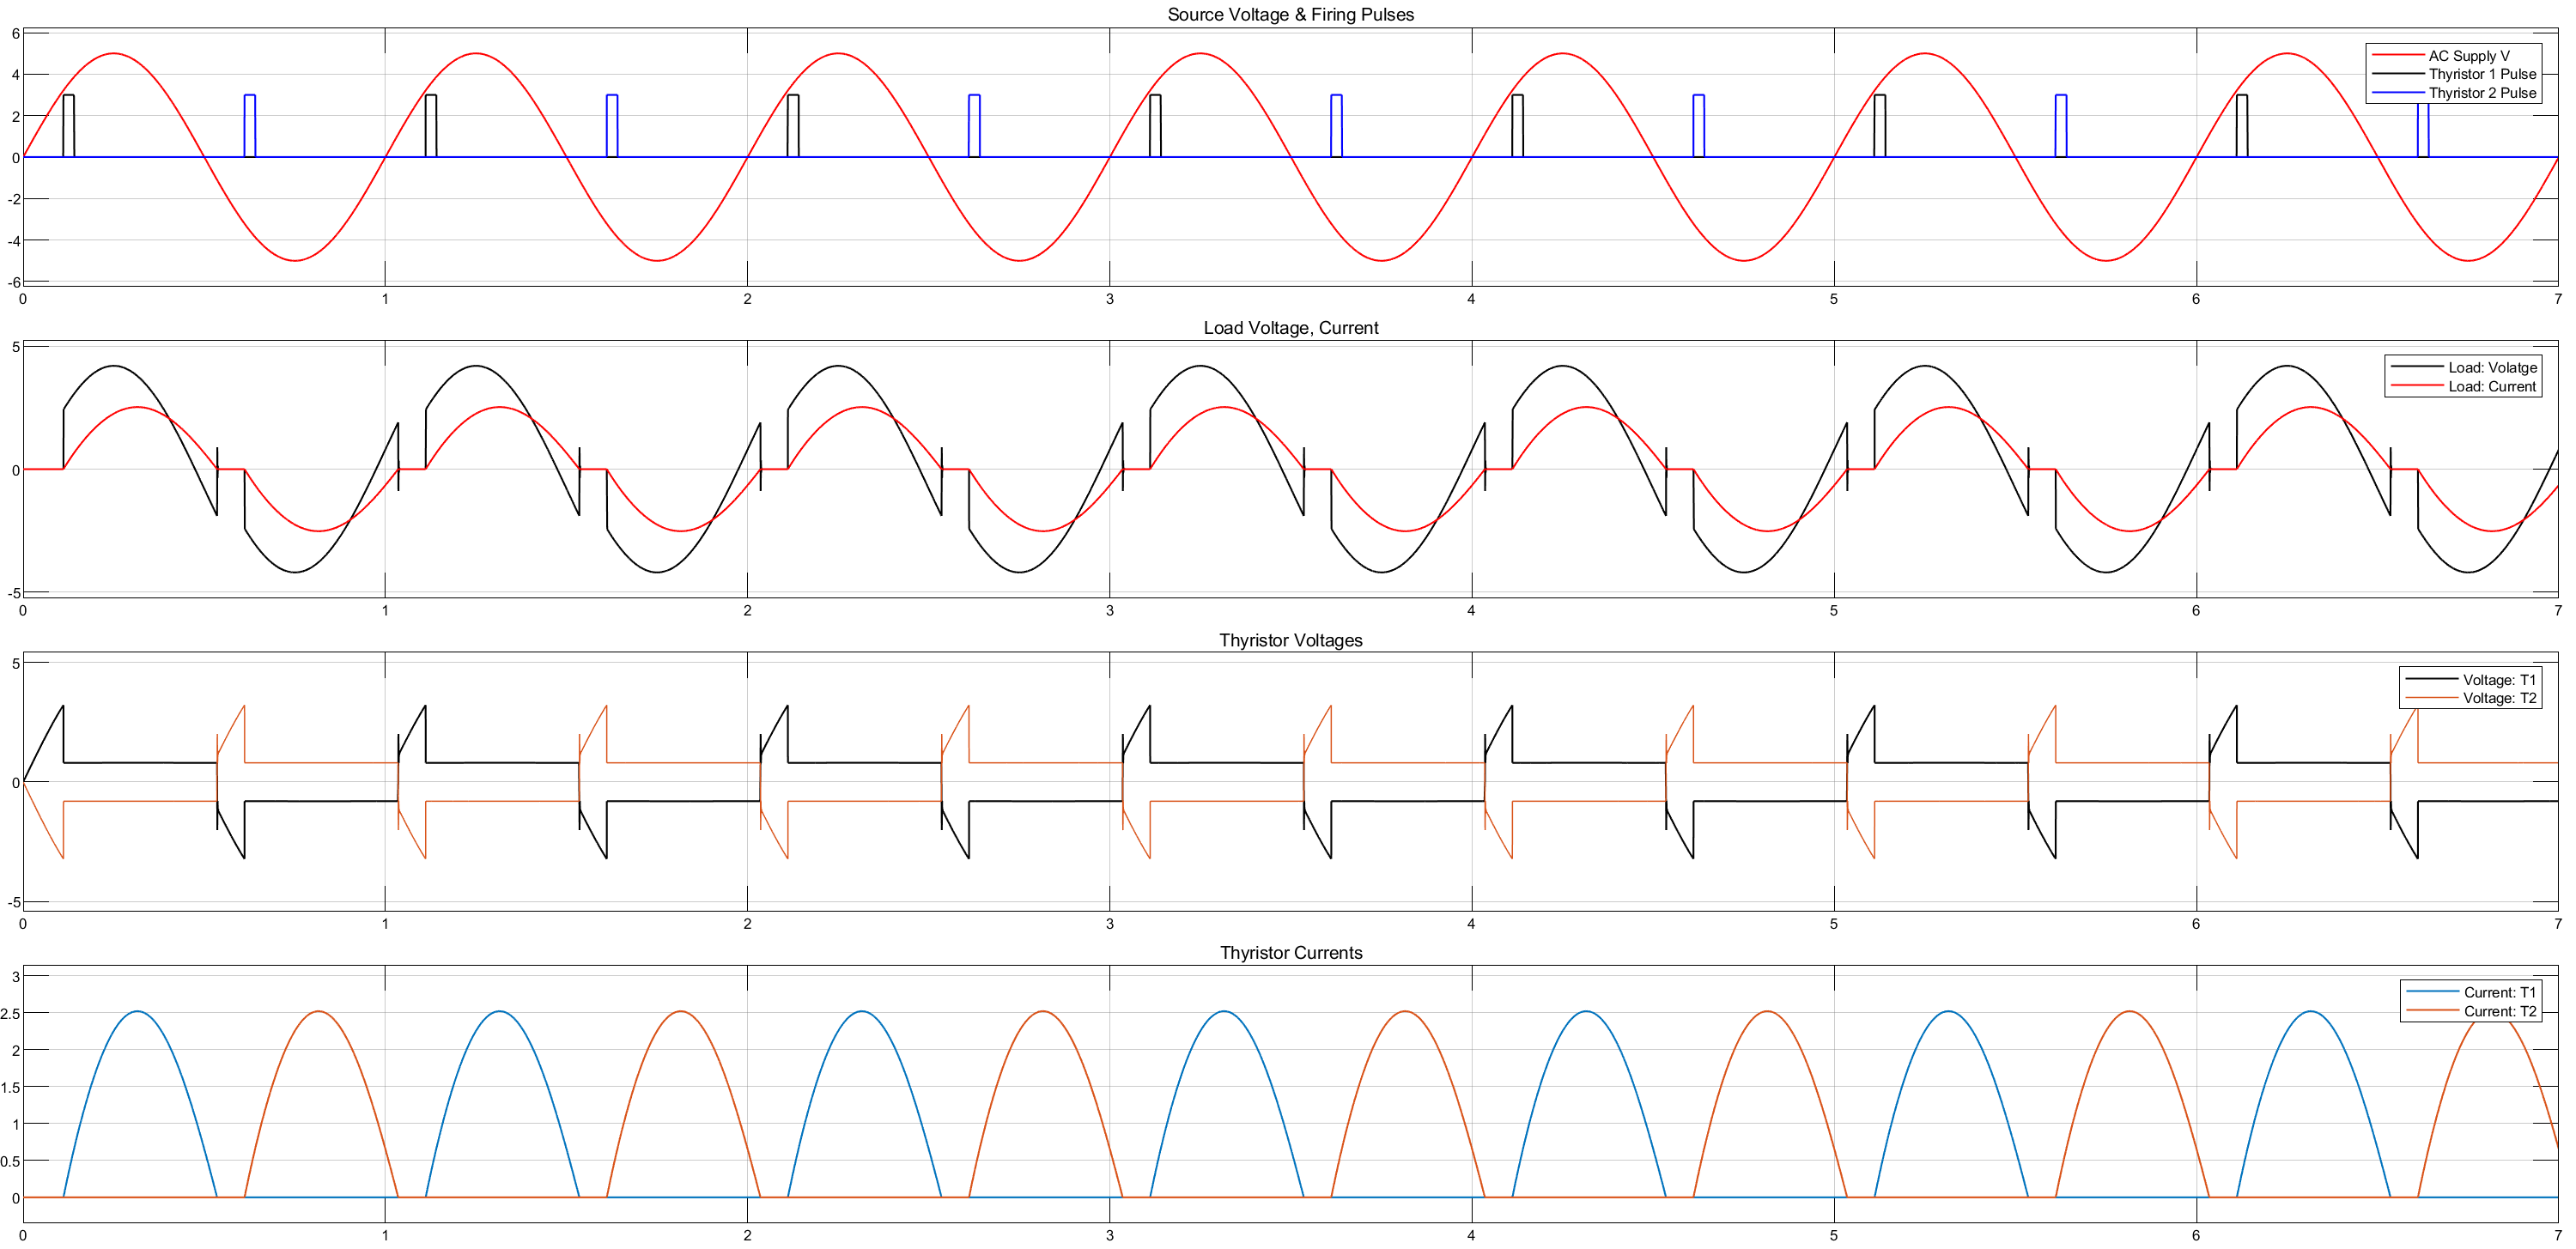
\includegraphics[width=\textwidth]{4RLd.png}
    \caption{Simulation Output for RL Load, AC-AC Bidirectional Voltage Controller}
    \label{fig:rlLoad}
\end{figure}


\section*{Discussion}
\addcontentsline{toc}{section}{Discussion}
The Buck Converter is a versatile DC-DC power electronic circuit widely used in various applications. Through MATLAB/Simulink simulations, we analyzed the relationship between the duty cycle of the PWM signal and the output voltage. The results demonstrate that the output voltage is directly proportional to the duty cycle, with higher duty cycles resulting in higher output voltages. For Continuous Conduction Mode (CCM), the inductor current remains smooth and does not fall to zero, ensuring efficient operation. In Discontinuous Conduction Mode (DCM), the inductor current falls to zero during part of the switching cycle, leading to increased ripple and reduced efficiency. These observations highlight the importance of proper component selection and PWM control for achieving optimal performance in Buck Converter applications.

\section*{Conclusion}
\addcontentsline{toc}{section}{Conclusion}
The study of the Buck Converter using MATLAB/Simulink simulations provides valuable insights into its operation and performance. The simulations confirm the theoretical principles of the Buck Converter, including the relationship between duty cycle, output voltage, and inductor current. The circuit effectively steps down the input voltage to the desired level with high efficiency, making it suitable for applications such as power supplies, battery chargers, and voltage regulation in electronic devices. The results emphasize the importance of understanding the operating modes and selecting appropriate components to optimize the converter's performance for specific applications.

\bibliographystyle{IEEEtran}
\renewcommand{\bibname}{References}
\addcontentsline{toc}{section}{References}
\bibliography{ref}

\end{document}
